\documentclass[11pt]{article}
\usepackage[margin=1in]{geometry}
\usepackage{amsmath,amssymb,booktabs,graphicx,microtype,longtable}
\usepackage[font=small,labelfont=bf]{caption}
\usepackage[hidelinks]{hyperref}
\graphicspath{{figures/v2/}}
% Generated by scripts/build_publication_release.py; do not edit.
% Source commit: 33829cf176eb41a780f318e2fe2fc335dfa32437
\newcommand{\AnalysisTimestamp}{2026-08-28T20:00:42Z}
\newcommand{\TotalSourceRecords}{164,209}
\newcommand{\DatasetCount}{13}
\newcommand{\ConfirmedPlanets}{6,354}
\newcommand{\HostSystems}{4,764}
\newcommand{\ConservativeHZ}{174}
\newcommand{\SmallConservativeHZ}{15}
\newcommand{\SmallHZMeasuredMass}{1}
\newcommand{\MeasuredMasses}{2,240}
\newcommand{\MeasurementLinks}{89,131}
\newcommand{\SelectedStars}{114,105}
\newcommand{\ObservedCandidates}{89}
\newcommand{\LatentCandidates}{54}
\newcommand{\EffectiveStars}{78.3}
\newcommand{\OccurrenceMedian}{0.692}
\newcommand{\OccurrenceLow}{0.267}
\newcommand{\OccurrenceHigh}{1.918}
\newcommand{\EarthPivotSelectionPercent}{0.00198}
\newcommand{\EarthPivotOnePer}{50,535}
\newcommand{\CompositionPlanets}{3,852}
\newcommand{\IndependentMasses}{679}
\newcommand{\CompositionMedianSpan}{0.251}
\newcommand{\ClimateInferred}{815}
\newcommand{\ClimateRobustInside}{22}
\newcommand{\ClimateSensitive}{16}
\newcommand{\EnvironmentTargets}{60}
\newcommand{\EscapeSupported}{43}
\newcommand{\AtmosphereMeasurements}{8,309}
\newcommand{\AtmosphereScenarios}{54}
\newcommand{\HwoStars}{12,944}
\newcommand{\HwoSupportedPlanets}{694}
\newcommand{\InformationActions}{6}
\newcommand{\InformationRows}{83}
\newcommand{\VenusESI}{0.874}

\title{Finding Earth 2.0: From the Observed Exoplanet Catalogue to\\Selection-Corrected Temperate Terrestrial Planet Inference}
\author{Biswajit Jana}
\date{Version 2.1.0 --- 19 September 2026}
\newcommand{\observed}{\textsc{Observed}}
\newcommand{\inferred}{\textsc{Model-Inferred}}
\newcommand{\simulated}{\textsc{Simulated}}
\newcommand{\scenario}{\textsc{Scenario-Assumption}}

\begin{document}
\maketitle
\begin{abstract}
The public exoplanet catalogue is a record of what surveys could detect and
validate, not a direct census of planetary systems. We connect
\TotalSourceRecords\ provenance-tracked source records to \ConfirmedPlanets\
confirmed planets and a separate Kepler DR25 selection-corrected inference.
The catalogue contains \ConservativeHZ\ planets in a nominal conservative
habitable zone and \SmallConservativeHZ\ also smaller than 1.6 Earth radii;
only \SmallHZMeasuredMass\ has an independently measured mass. In a fixed
50--500 day, 0.5--2 Earth-radius DR25 box, the model gives
\OccurrenceMedian\ planets per selected star (95\% interval
\OccurrenceLow--\OccurrenceHigh). Observations, model inferences, simulations,
and mission assumptions remain separate. A Solar-System control gives Venus an
Earth Similarity Index of \VenusESI, falsifying any interpretation of
similarity as habitability. This work ranks evidence and missing measurements;
it does not estimate the probability of life.
\end{abstract}

\section{Introduction}
Thousands of confirmed planets make ``Earth 2.0'' sound like a catalogue
lookup. It is an inverse problem: transit geometry, observing windows, pipeline
recovery, vetting, follow-up, and publication all shape the visible sample. A
similar radius or incident flux does not establish a rocky interior, retained
atmosphere, temperate surface, or biology.

Each claim receives one of four labels: \observed\ for archive measurements;
\inferred\ for results conditional on a model; \simulated\ for validation or
prospective experiments; and \scenario\ for instrument or physical assumptions.

\section{Scientific Question}
We ask which known planets satisfy stated terrestrial-size and temperate-orbit
criteria; how much of the population the survey could have hidden; which
interpretations survive changes in composition, climate, and stellar models;
and which next observation should reduce the most decision-relevant uncertainty.
No datum in this project answers whether life exists elsewhere.

\section{Public Data}
The archive layer contains \DatasetCount\ retrievals totalling
\TotalSourceRecords\ records. The confirmed-planet analysis covers
\ConfirmedPlanets\ planets around \HostSystems\ hosts, with
\MeasurementLinks\ measurement-to-publication links. NASA Exoplanet Archive
tables supply planetary, stellar, candidate, TCE, and atmospheric products;
Gaia DR3 supplies astrometric checks; MAST and DACE support deep dives; MIST
supplies stellar tracks; and HPIC supports direct-imaging scenarios
\cite{NasaExoplanetArchive,NasaExoplanetArchivePS,GaiaDR3,Choi2016}.
Every retrieval records query text, timestamp, URL, row count, and SHA-256. The
v2 bundle redistributes derived products and manifests, excluding controlled
source rows and upstream model archives.

\section{Evidence Architecture}
A normalized evidence graph connects systems, planets, aliases, measurements,
publications, archive rows, and derived claims. Exact identifiers take priority
over names. Dependency paths prevent an inferred mass from silently becoming
independent evidence for density or escape velocity. Category boundaries are
carried from records to figures, the website, and this paper.

\section{Selection Function}
The DR25 model separates geometry, observing window, pipeline recovery, and
vetting, while respecting that pipeline completeness already includes the
window. Injection experiments calibrate recovery. Target-isolated folds,
monotonicity tests, and a pinned KeplerPORTs regression constrain errors.
At an Earth-period, Earth-radius pivot, mean total selection is
\EarthPivotSelectionPercent\%, roughly one selected signal per
\EarthPivotOnePer\ searched stars. This explains sparsity; it is not the
population estimator.
\begin{figure}[ht]
\centering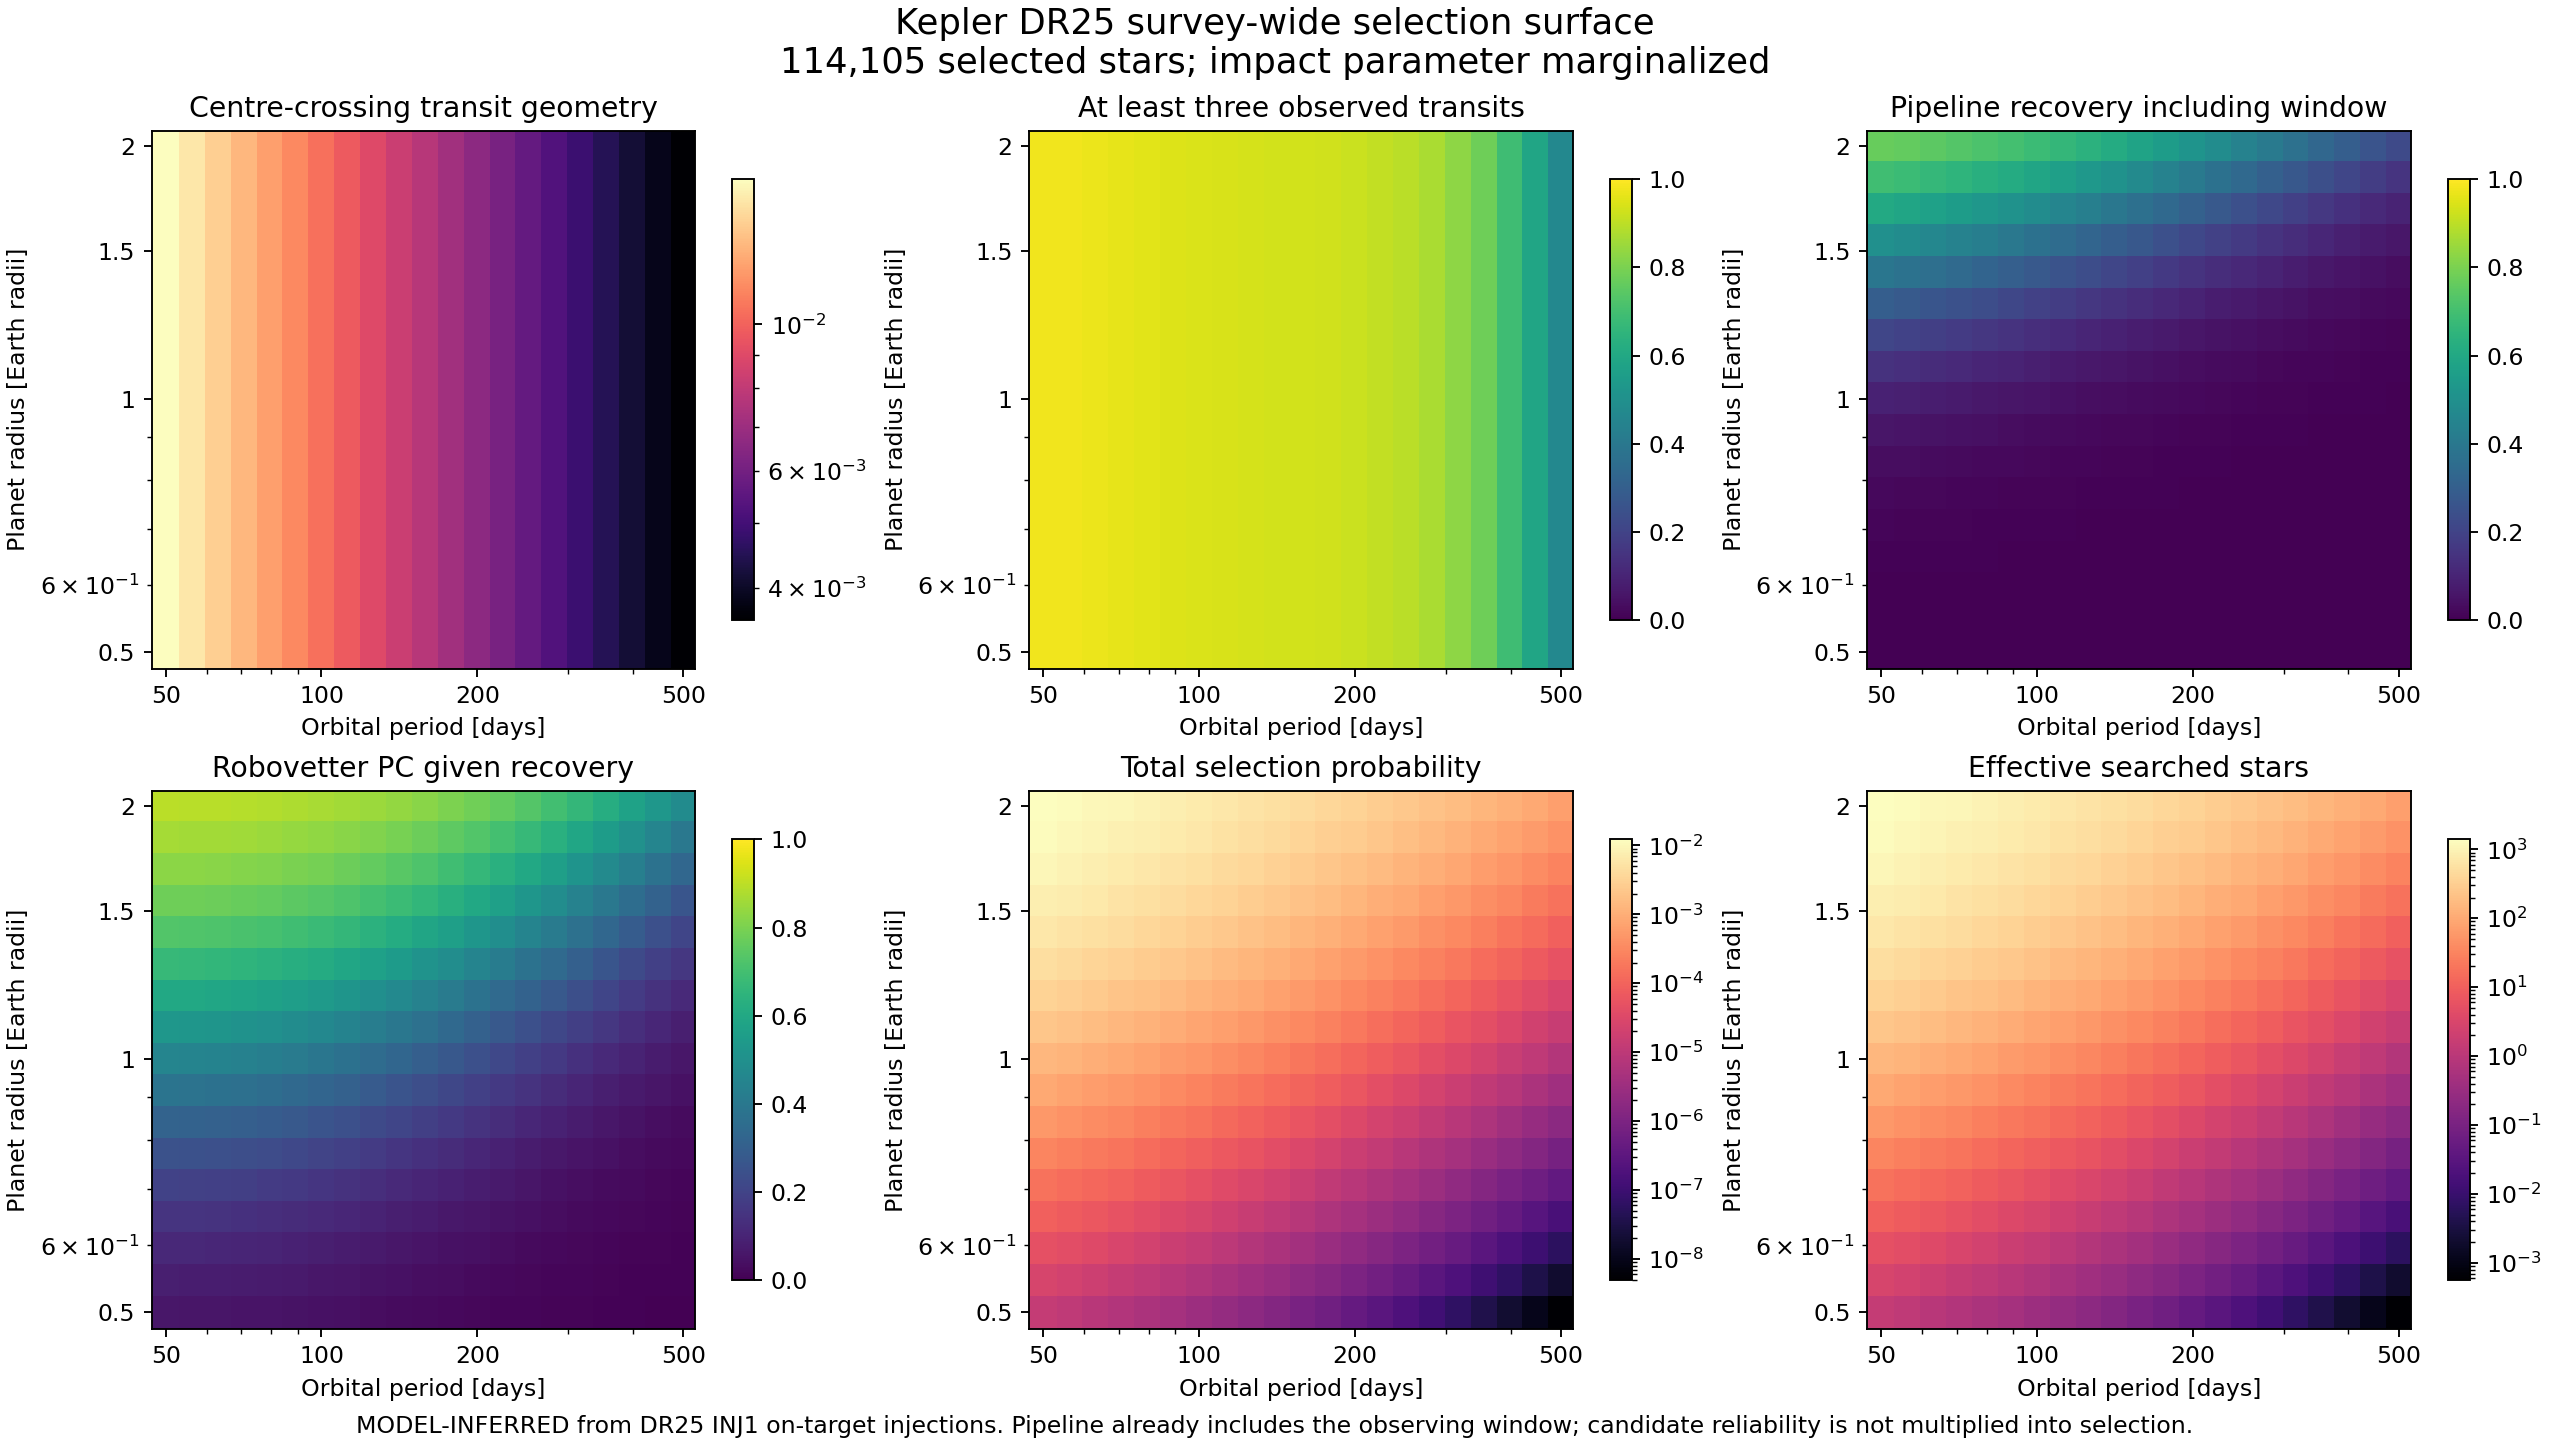
\includegraphics[width=.92\linewidth]{dr25_selection_surface.png}
\caption{\inferred\ total selection over the declared DR25 domain.}
\end{figure}

\section{Population Model}
The population is an inhomogeneous Poisson process in log period and log radius,
with a normalized power-law shape and integrated rate. Reliability and
astrophysical false-positive uncertainty propagate through shared draws. The
contract includes \SelectedStars\ stars and \ObservedCandidates\ candidates;
reliability implies about \LatentCandidates\ latent valid candidates. The fitted
shape corresponds to \EffectiveStars\ effective stars after selection weighting.
The fixed-box occurrence posterior is \OccurrenceMedian\
(\OccurrenceLow--\OccurrenceHigh) planets per selected star. It is conditional
on this population, domain, selection family, reliability model, and priors; it
is neither habitable-zone $\eta_\oplus$ nor a life probability.
\begin{figure}[ht]
\centering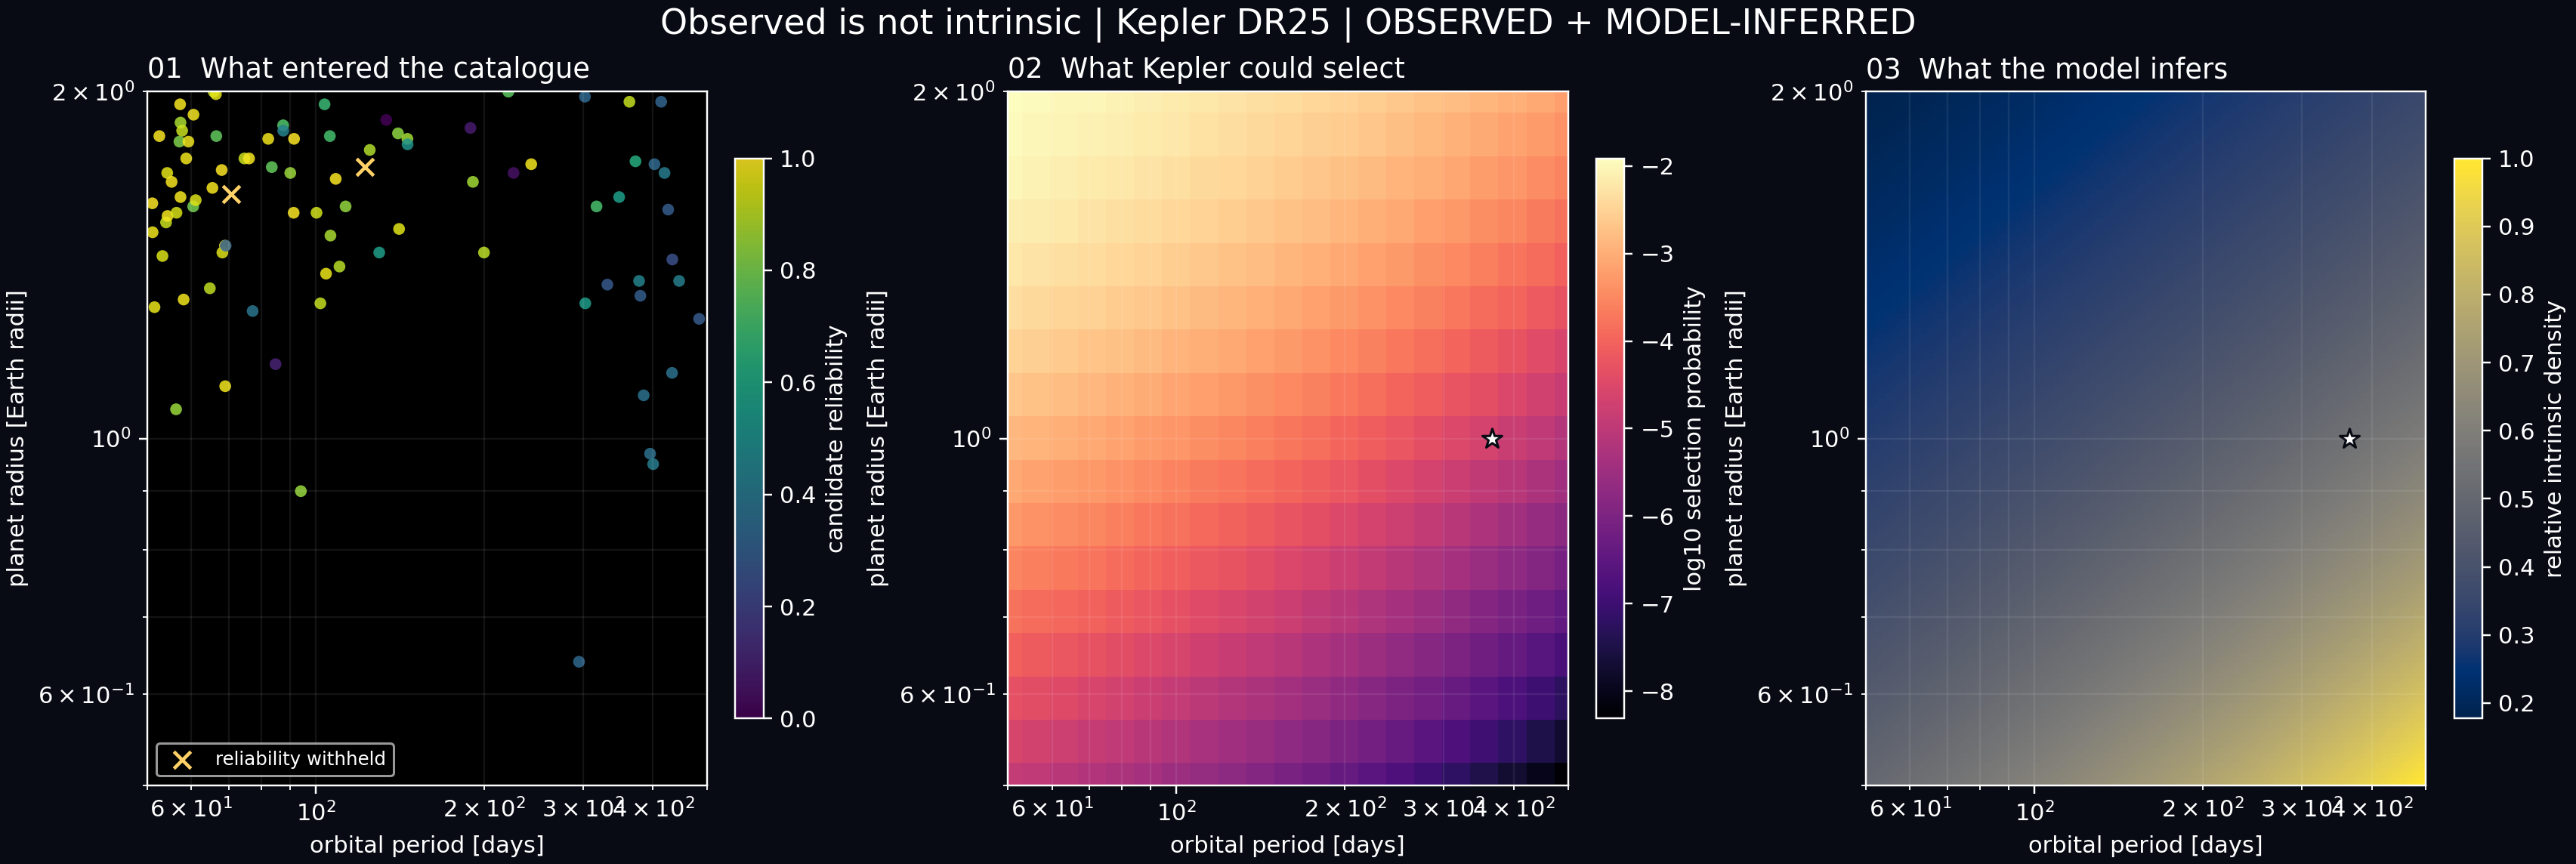
\includegraphics[width=.96\linewidth]{dr25_observed_vs_intrinsic.png}
\caption{Observed candidates, survey selection, and inferred population.}
\end{figure}

\section{Habitable Zone}
Instantaneous boundaries follow Kopparapu et al.
\cite{Kopparapu2013,Kopparapu2013Erratum}. Nominal classification finds
\ConservativeHZ\ confirmed planets inside conservative boundaries, including
\SmallConservativeHZ\ smaller than 1.6 Earth radii. This is a radiative climate
condition, not a measured surface state. Uncertainty propagates by Monte Carlo;
hosts outside the calibrated temperature domain are explicitly unsupported or
extrapolated.

\section{Composition}
The ensemble compares a Rogers radius baseline, Zeng iron-silicate envelope,
and Otegi rocky/volatile relations \cite{Rogers2015,Zeng2016,Otegi2020}.
It evaluates \CompositionPlanets\ planets, but only \IndependentMasses\ have
accepted independent masses for two-dimensional inference. Predictions,
$M\sin i$, and upper limits do not become dynamical masses. The median range
between model probabilities is \CompositionMedianSpan; that disagreement is
retained rather than averaged away.
\begin{figure}[ht]
\centering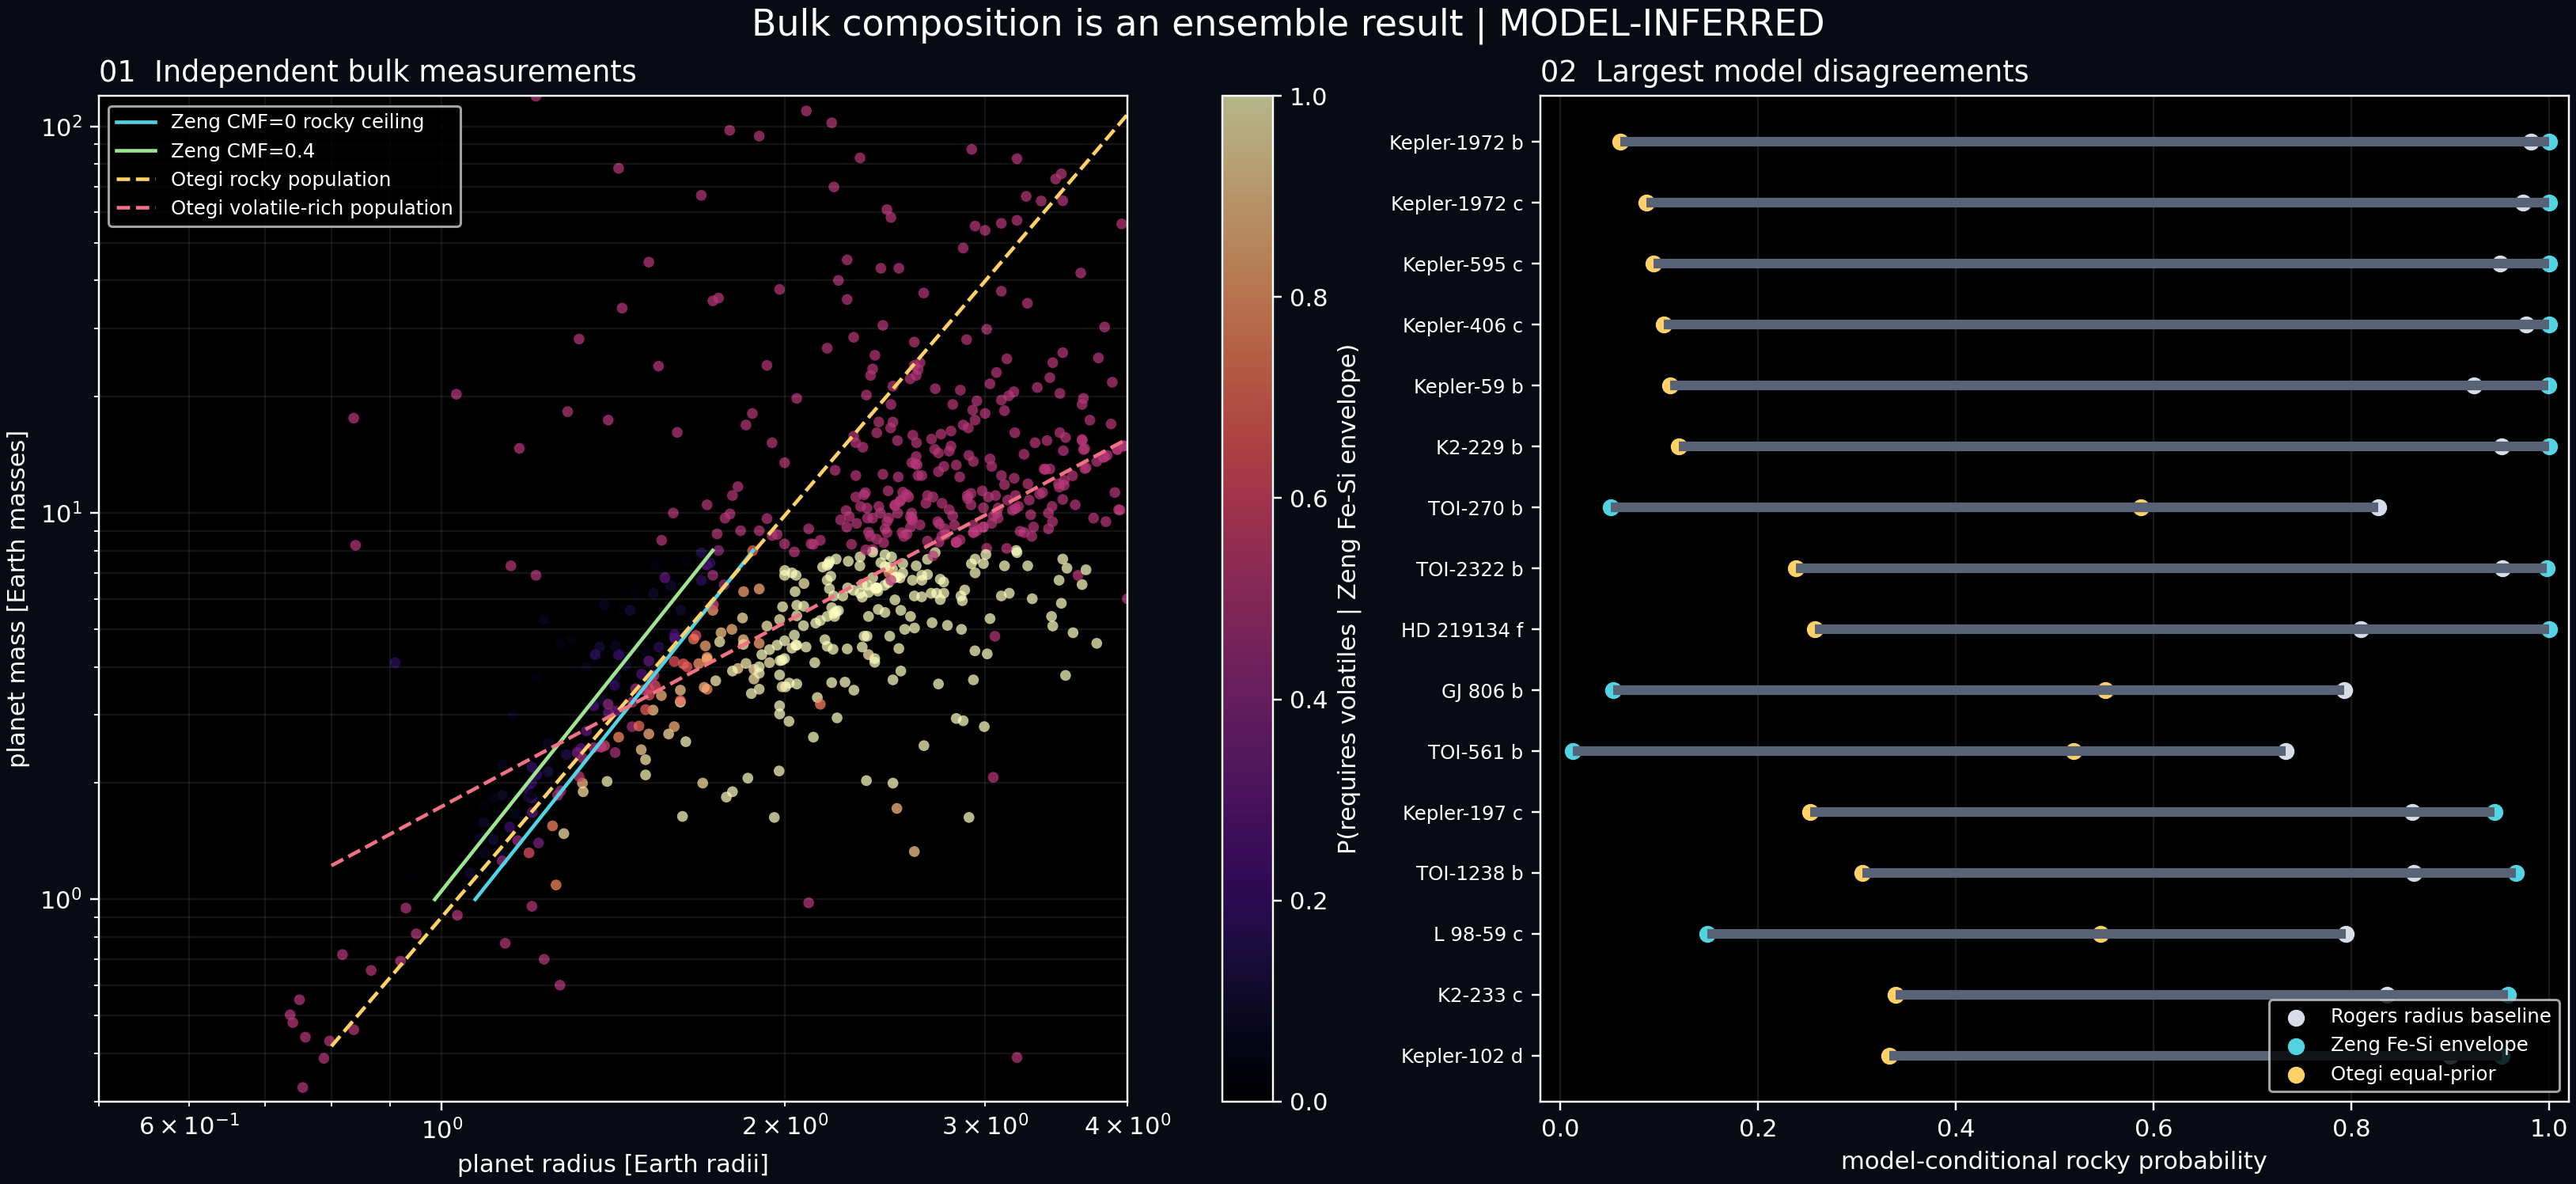
\includegraphics[width=.86\linewidth]{composition_model_disagreement.png}
\caption{\inferred\ composition-model disagreement and support.}
\end{figure}

\section{Stellar Environment}
High-energy forcing is separate from bolometric irradiation. For
\EnvironmentTargets\ terrestrial-size targets, age and activity measurements
support bounded XUV histories where possible; \EscapeSupported\ support escape
ensembles. Calculations vary heating efficiency, XUV radius, and initial envelope
fraction while holding planet properties fixed, so they are sensitivity
scenarios rather than atmospheric histories.

\section{Atmospheric Survival}
Retention depends on supply, forcing, chemistry, magnetic environment, and
nonthermal escape beyond the simplified model. The project reports cumulative
forcing and ranges rather than a retained/lost verdict. The evidence layer
indexes \AtmosphereMeasurements\ spectral measurements while keeping
\AtmosphereScenarios\ supported clear, isothermal observability scenarios
distinct from detections. Reduction comparisons are never averaged into a
preferred atmosphere.

\section{Observability}
Transmission signals use declared molecular weight, temperature, gravity, and
scale heights. Direct-imaging calculations sample phase, orientation,
eccentricity, albedo, and working angles. They ask whether a signal could be
measured under a scenario, not whether an atmosphere exists. This distinction
also separates non-transiting nearby imaging targets from transiting targets.

\section{Future Missions}
The observatory tracks Gaia, JWST, Roman, PLATO, ANDES, and HWO against distinct
questions; it defines no cross-mission merit score. The HWO precursor atlas has
\HwoStars\ stellar rows and supports calculations for
\HwoSupportedPlanets\ known planets. Unknown inclinations and orbital geometry
are sampled, with assumptions visible beside every probability.
\begin{figure}[ht]
\centering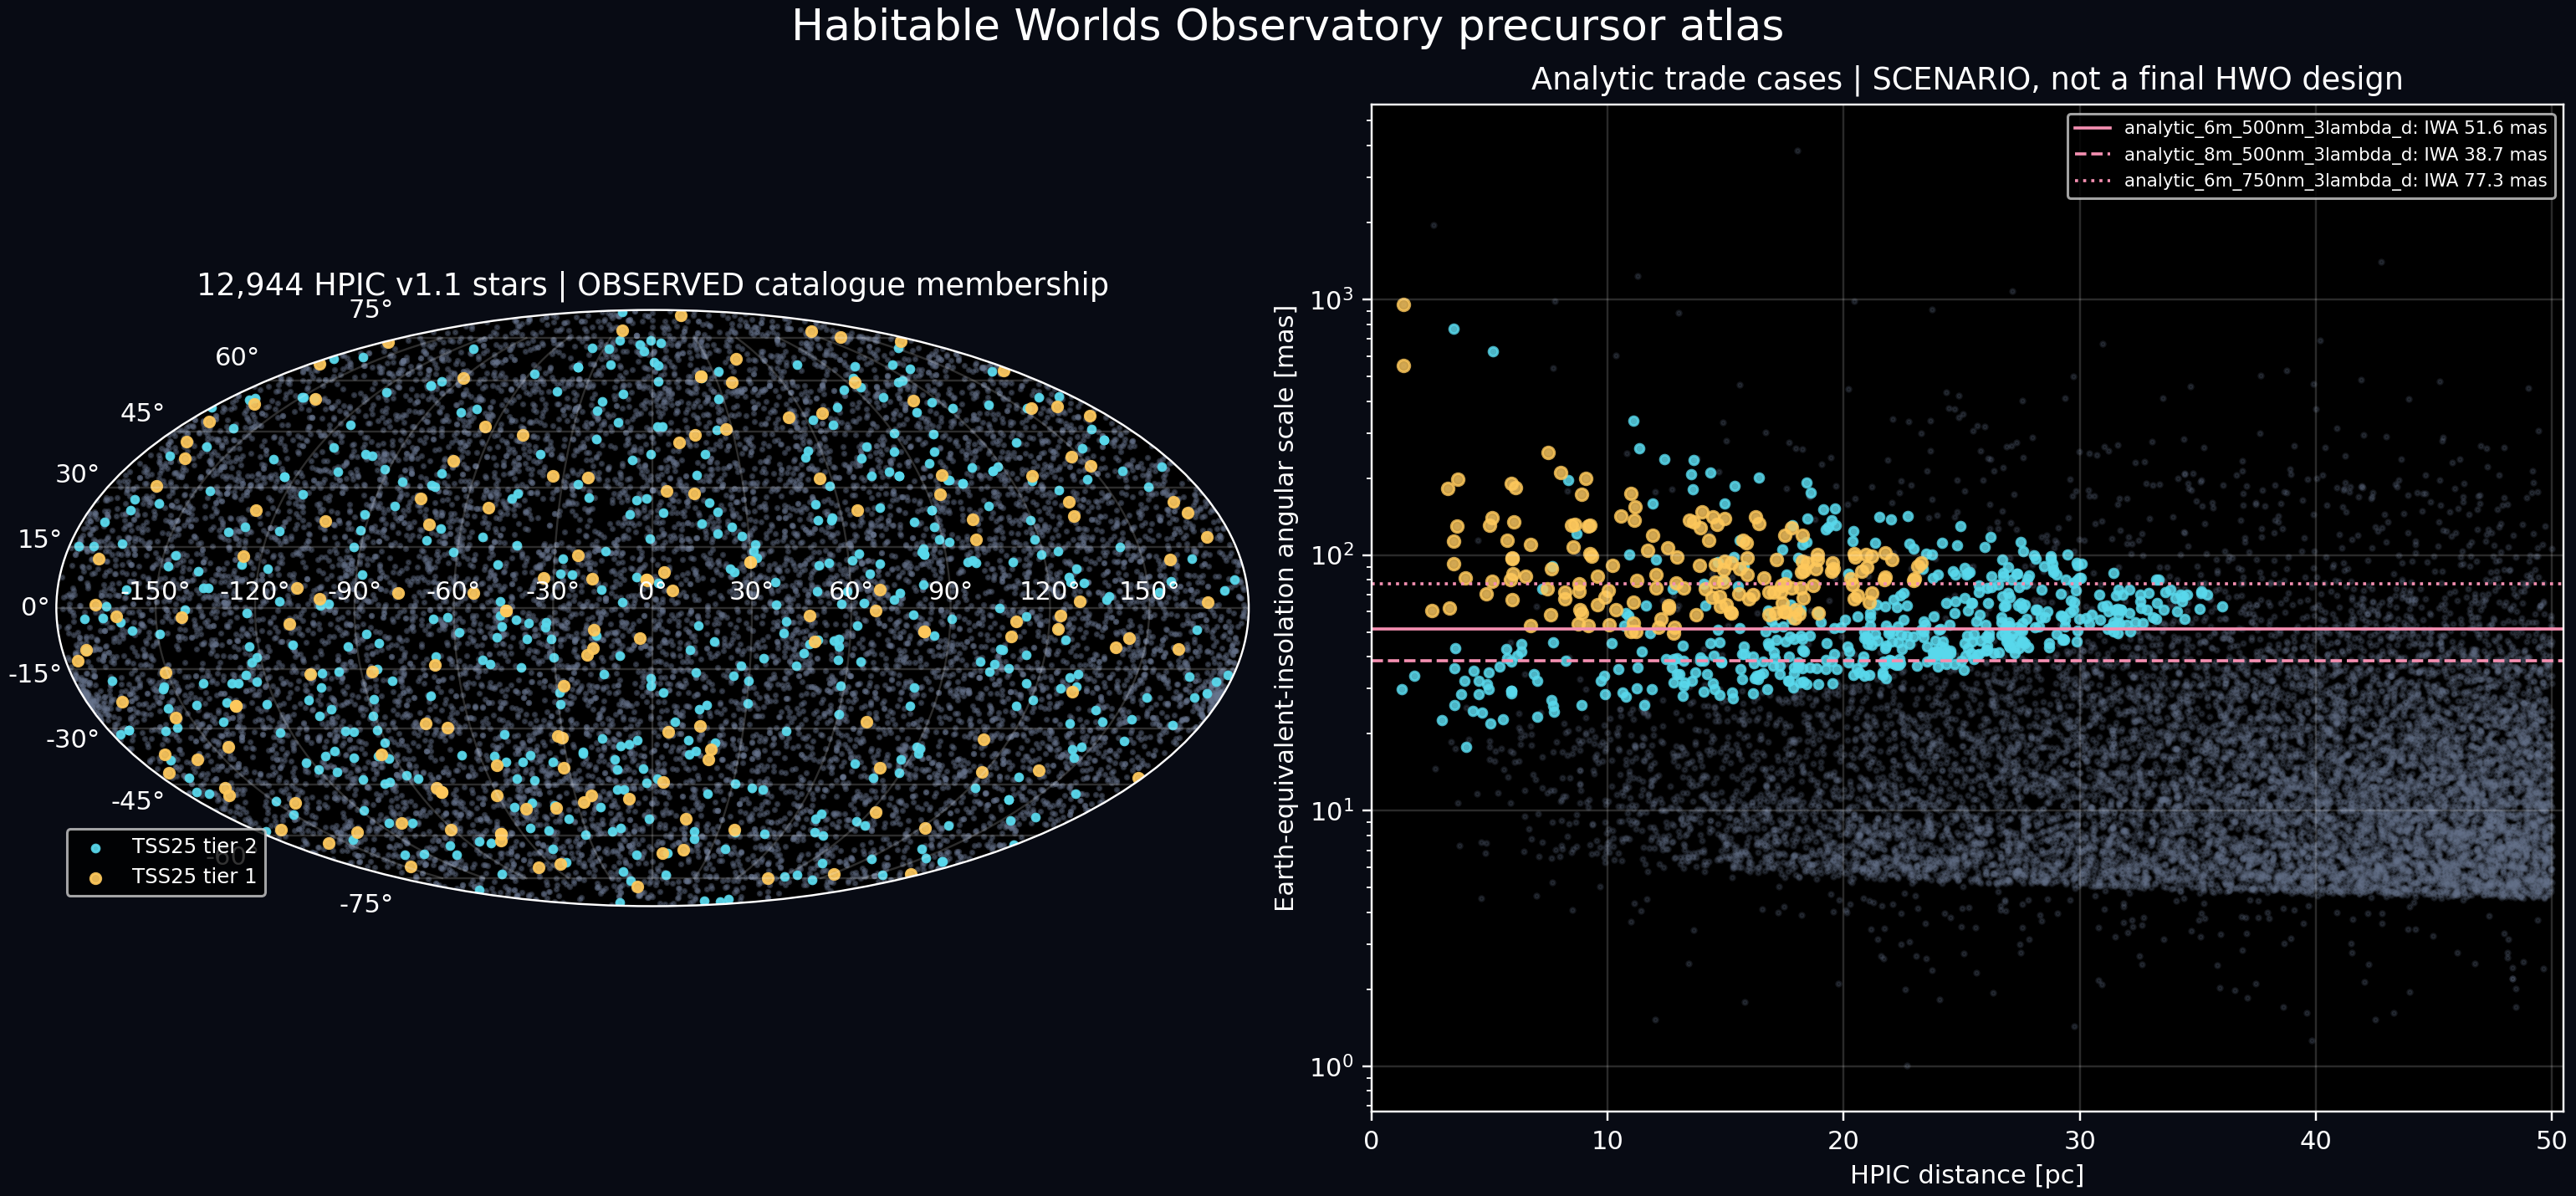
\includegraphics[width=.9\linewidth]{hwo_precursor_atlas.png}
\caption{\scenario\ access under three instrument concepts, not mission yield.}
\end{figure}

\section{Bayesian Design}
Expected information gain (EIG) selects observations by expected posterior
change. For action $a$ and possible result $y$,
\[
\operatorname{EIG}(a)=\mathbb{E}_{y\sim p(y\mid D,a)}
\left[D_{\mathrm{KL}}\{p(\theta\mid D,y,a)\|p(\theta\mid D)\}\right].
\]
The experiment evaluates \InformationActions\ actions; only
\InformationRows\ target-action rows pass support contracts. Simplified
likelihoods are \simulated, so EIG compares specified experiments rather than
promising telescope performance.
\begin{figure}[ht]
\centering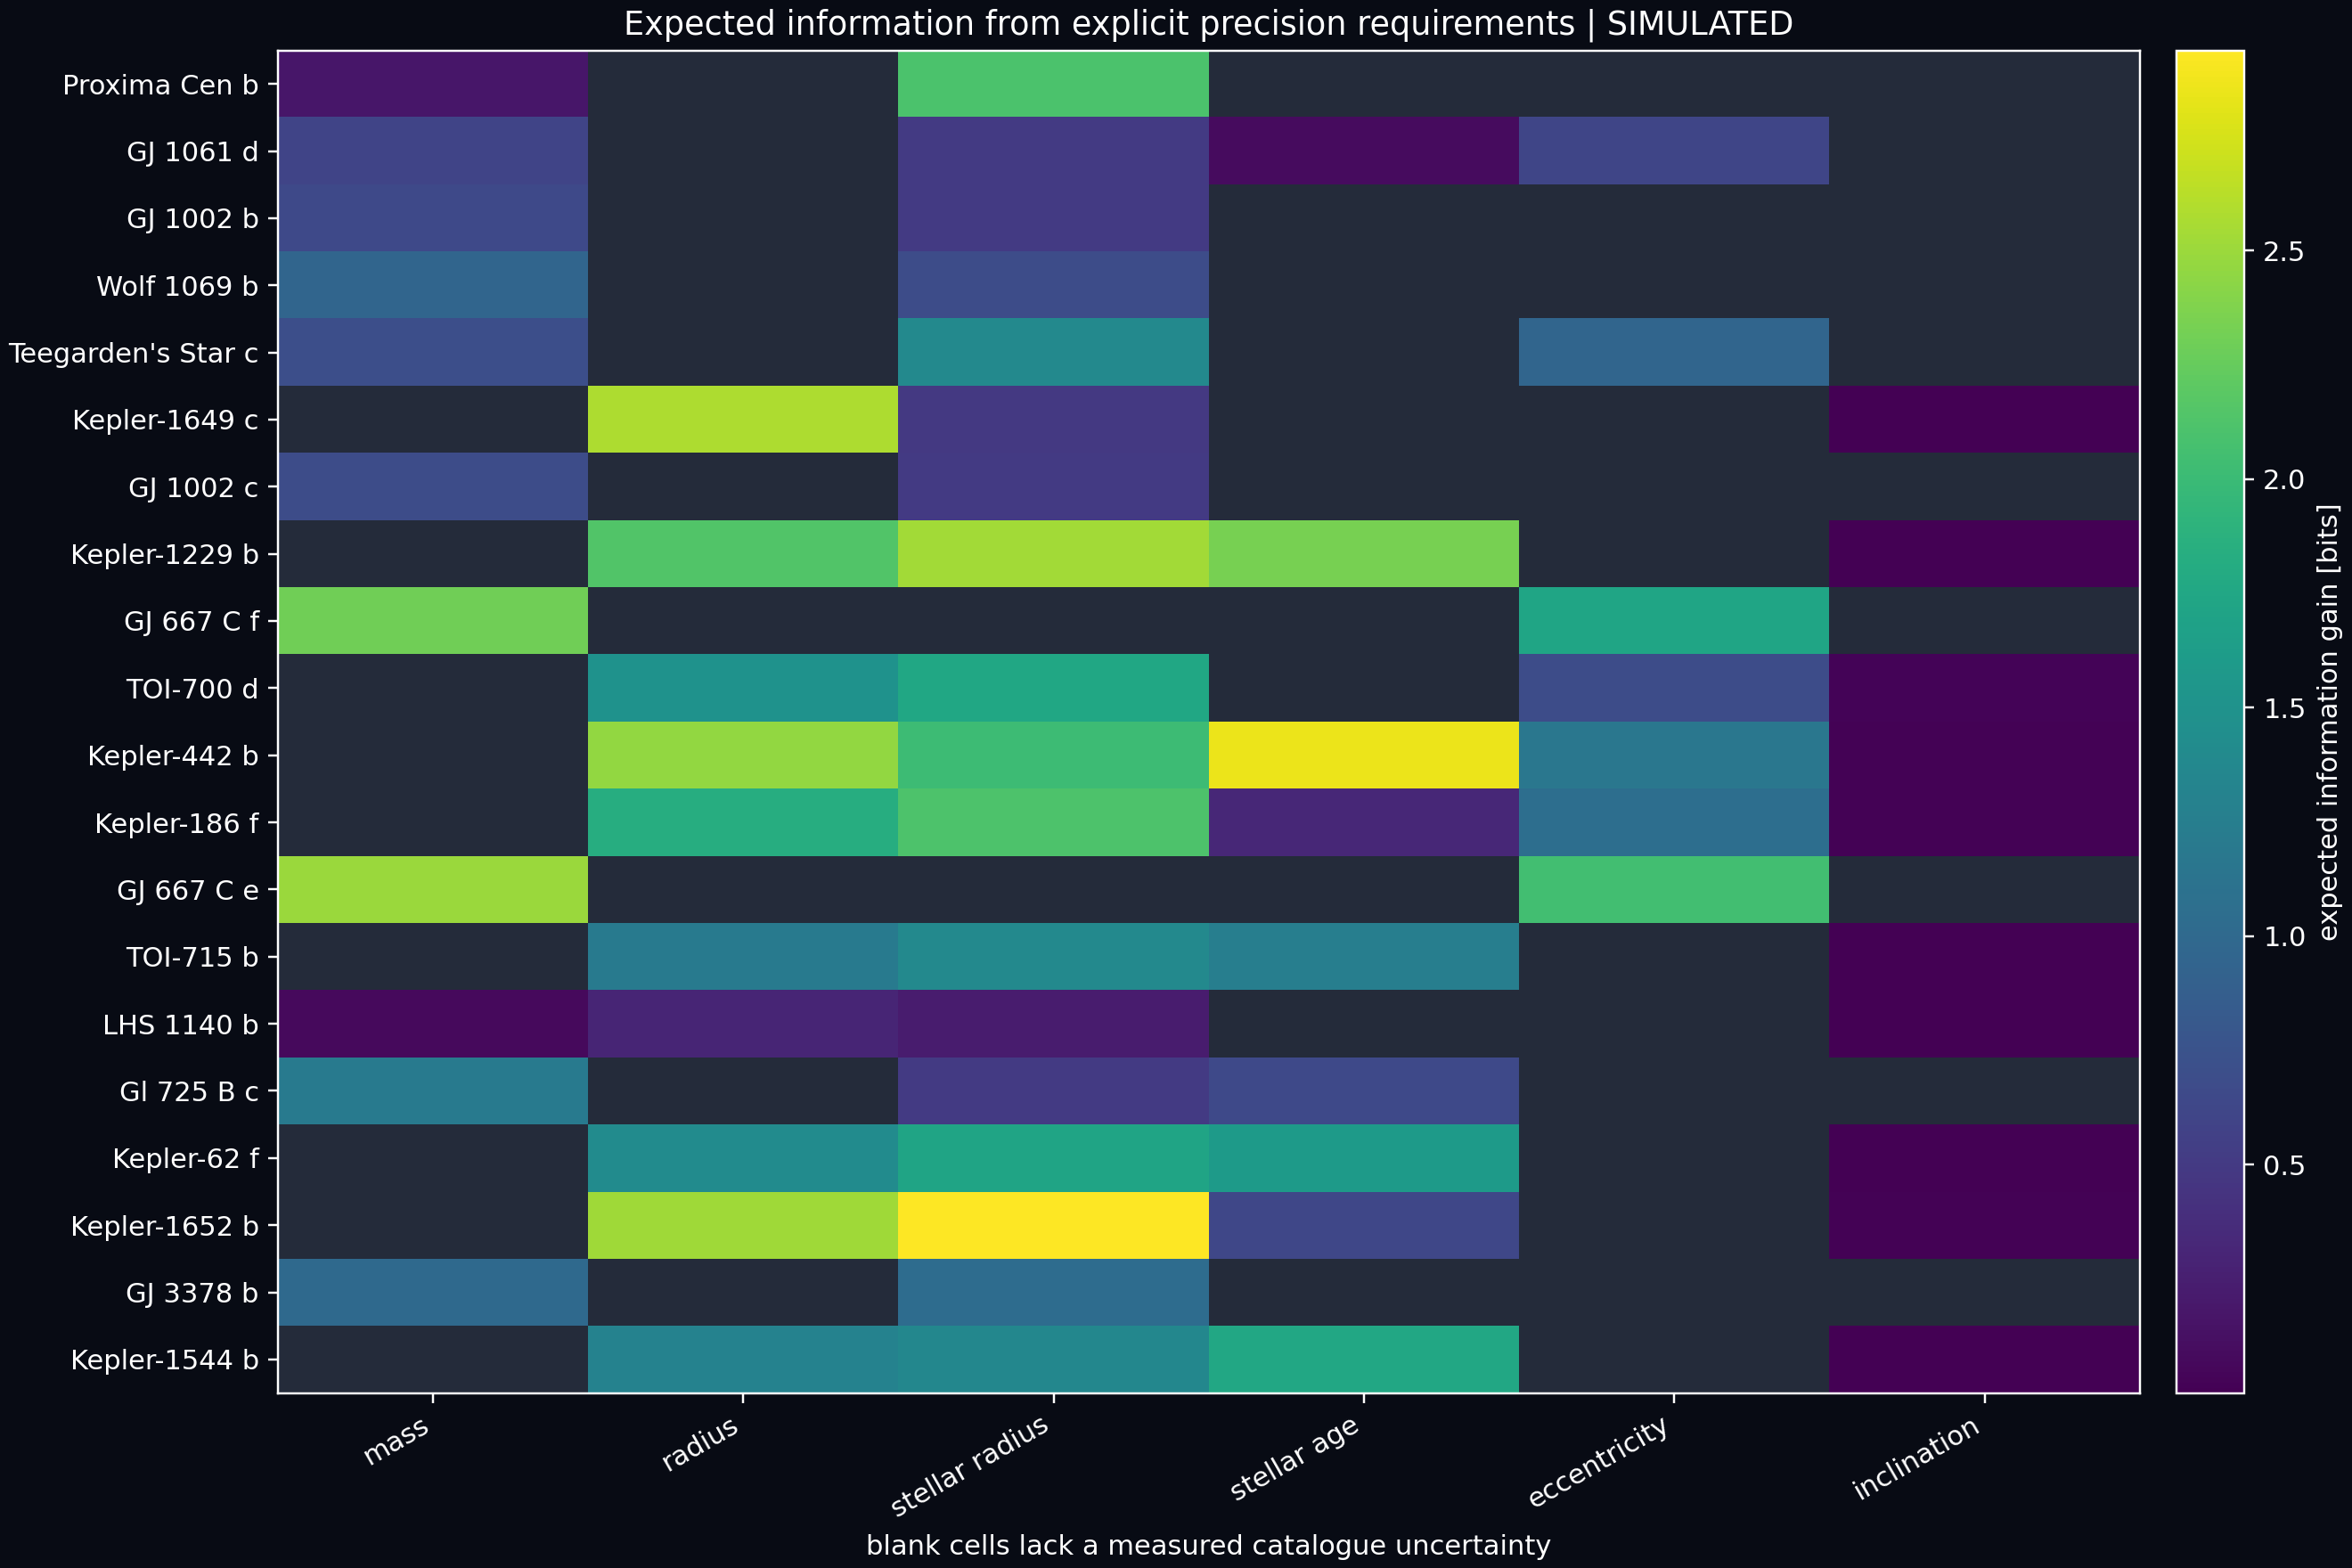
\includegraphics[width=.88\linewidth]{expected_information_gain.png}
\caption{\simulated\ action-specific EIG; missing means unsupported.}
\end{figure}

\section{Results}
The observed funnel narrows from \TotalSourceRecords\ source rows to
\ConfirmedPlanets\ confirmed planets, \ConservativeHZ\ nominal conservative-HZ
worlds, \SmallConservativeHZ\ small conservative-HZ worlds, and
\SmallHZMeasuredMass\ with an independent mass. Its message is measurement
scarcity, not discovery of another Earth. Selection correction changes the
scale but retains broad uncertainty. Only \ClimateInferred\ planets support
time-dependent climate inference; \ClimateRobustInside\ remain robustly inside
across prescriptions and \ClimateSensitive\ are boundary- or model-sensitive.

\section{Robustness}
Synthetic recovery covers flat, power-law, Earth-box, low-completeness,
finite-injection, reliability, and stellar-radius cases. Deliberately broken
radius-law and halved-completeness tests expose misspecification rather than
passing silently. Candidate results are also recomputed across score weights,
composition models, climate boundaries, escape assumptions, and instruments.

\section{Solar-System Falsification}
Earth, Venus, Mars, Mercury, and Jupiter test model behavior outside population
counts. Venus receives ESI \VenusESI\ while its conservative-HZ probability is
zero. The control therefore falsifies any reading of ESI as habitability.
\begin{figure}[ht]
\centering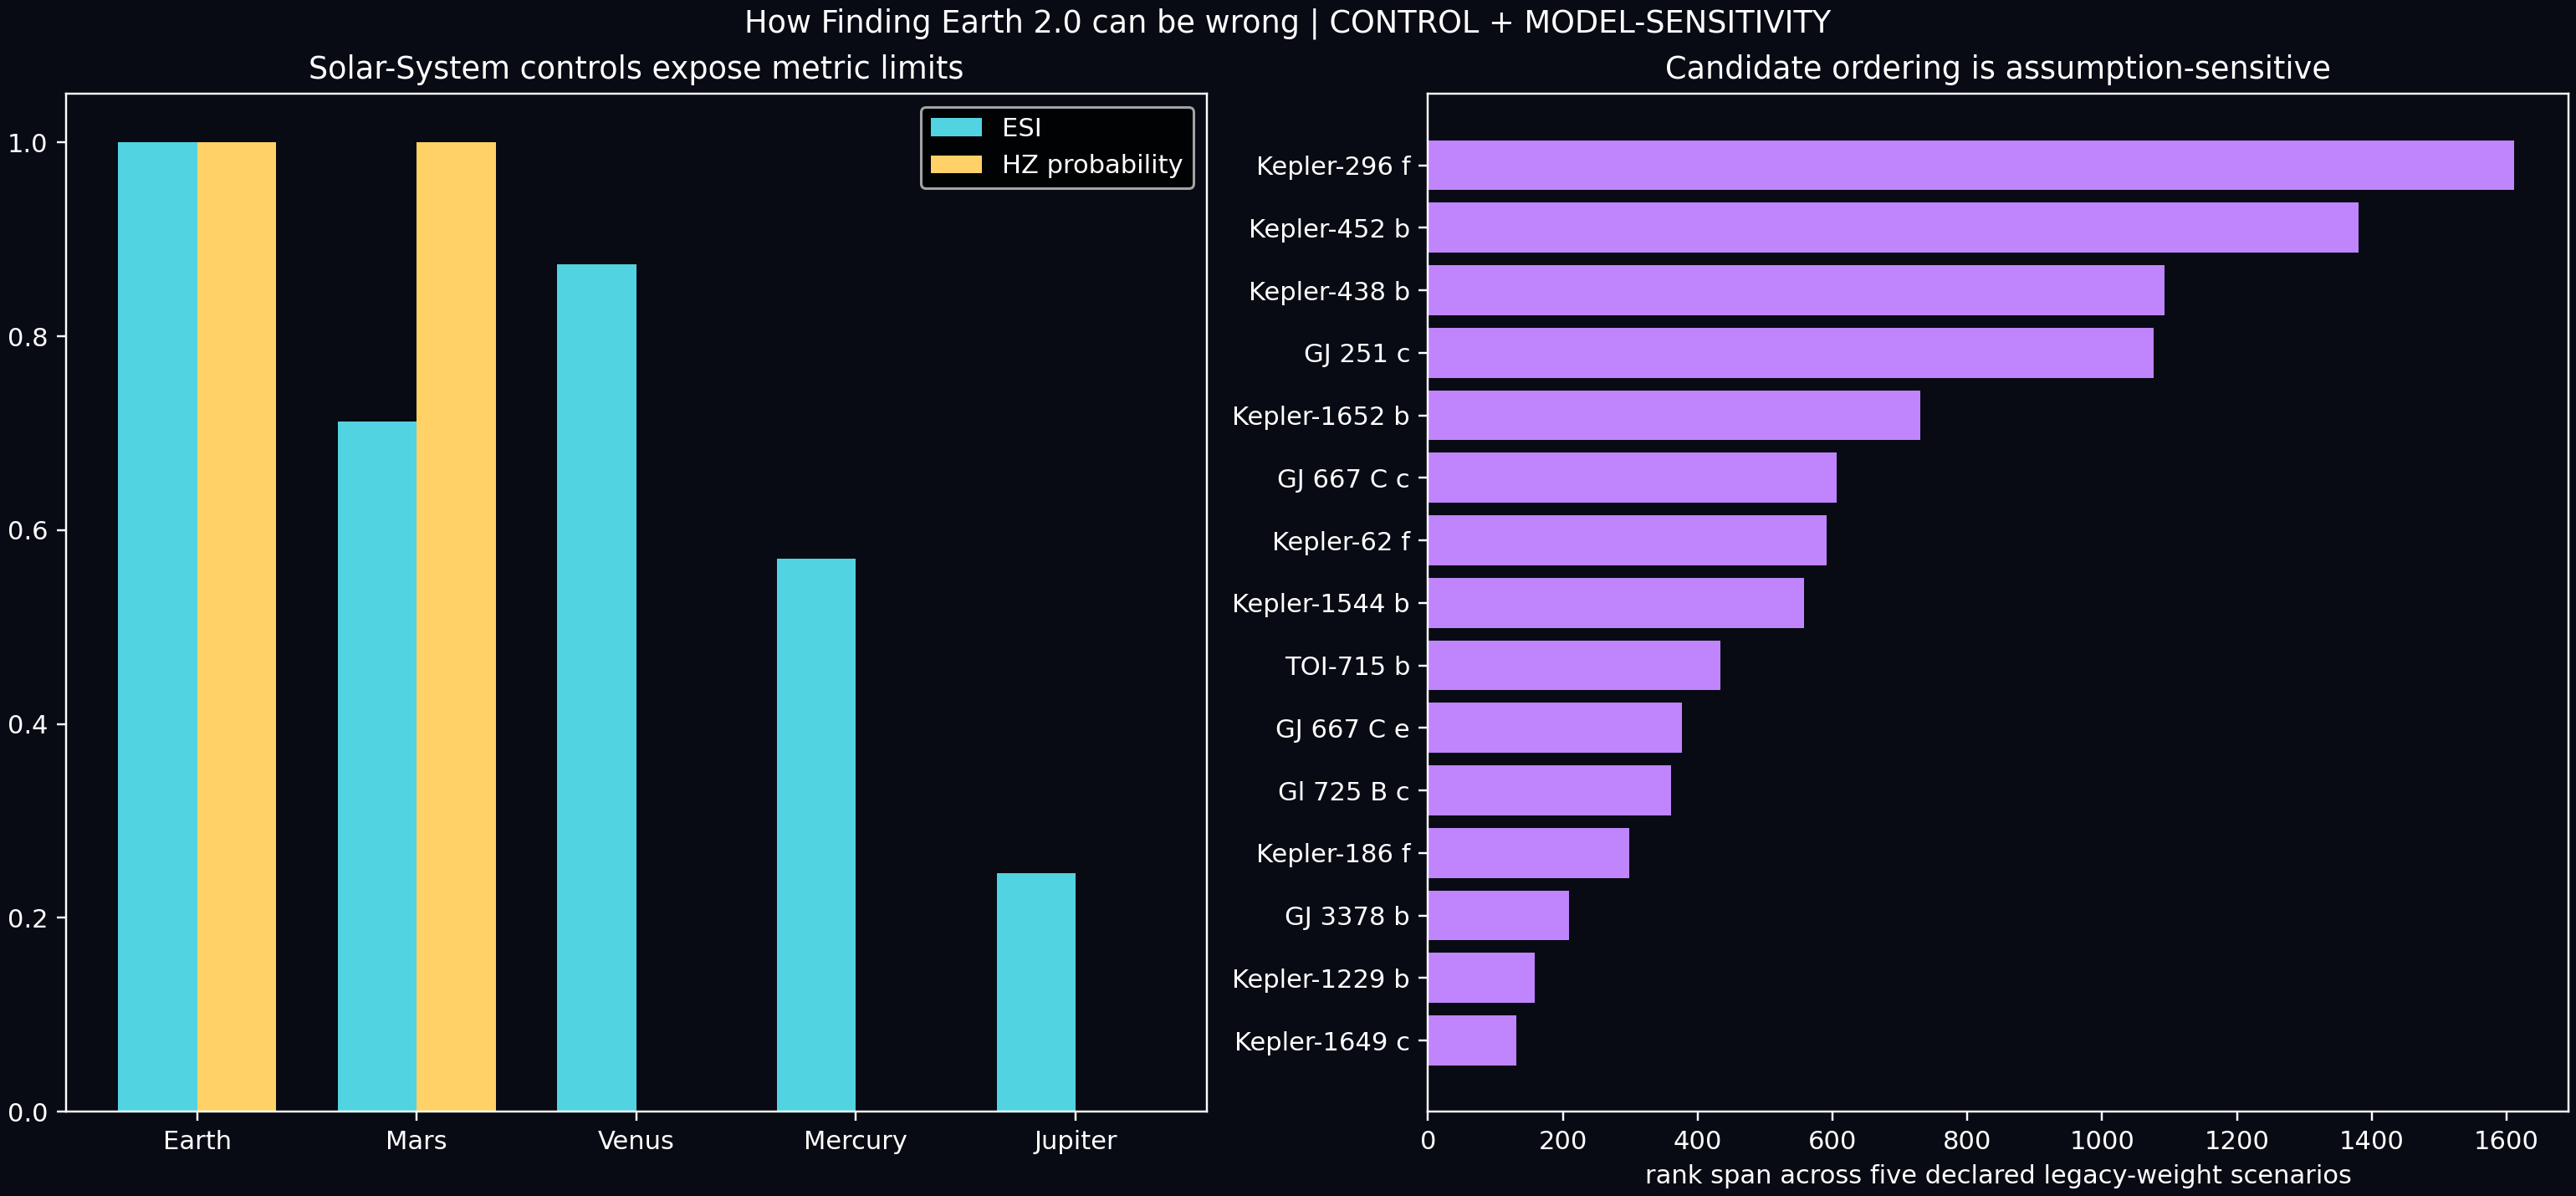
\includegraphics[width=.9\linewidth]{falsification_and_robustness.png}
\caption{Observed Solar-System controls and model-sensitivity tests.}
\end{figure}

\section{Limitations}
Occurrence is conditional on one stellar selection, one constrained selection
family, reliability inputs, priors, and a simple population shape. Catalogue
measurements remain heterogeneous. Bulk data do not identify unique interiors.
One-dimensional HZ boundaries omit clouds, oceans, geochemistry, rotation, and
composition. Escape models hold properties fixed. Observability omits full
retrieval systematics. Mission details can change. No biosignature model or life
prior is fitted.

\section{Discussion}
The project turns a ranking into falsifiable questions: what was observed, what
the survey could select, which model supplies each inference, how strongly the
answer changes, and which observation could reduce uncertainty. A compelling
target can have Earth-like orbit and radius while its mass, atmosphere, activity
history, and imaging geometry remain unknown. The honest output is then a
measurement recommendation rather than a stronger adjective.

\section{Conclusions}
The catalogue is not the Universe. The public record supports a small set of
temperate terrestrial-size candidates, but the funnel ends with only
\SmallHZMeasuredMass\ independent mass. Selection-aware inference reveals a
larger, uncertain underlying population while preserving the boundary between
occurrence and habitability. The v2 release makes headline values traceable,
publishes assumptions beside results, rejects overclaiming with controls, and
identifies observations with the greatest expected value.

\appendix
\section{Equations and Computational Contract}
ESI is a weighted geometric combination of bounded similarity transforms.
Asymmetric errors propagate through deterministic-seed Monte Carlo draws. HZ
fluxes follow published temperature polynomials. The occurrence likelihood is
evaluated in $d\ln P\,d\ln R$ and normalized over the fixed domain.

\section{Provenance and Reproduction}
The analysis timestamp is \texttt{\AnalysisTimestamp}. Run
\texttt{python -m earth2 report}, phase builders, and
\texttt{python scripts/build\_publication\_release.py}. Verify
\texttt{MANIFEST.sha256}; \texttt{SOURCE\_COMMIT} records the exact source state.

\section{Prior and Model Sensitivity}
Posterior samples and reliability endpoints are released. Composition remains
model-specific. Climate reports agreement across three prescriptions. Escape,
albedo, orbit, and instrument assumptions remain explicit dimensions.

\section{Completeness and Reliability Diagnostics}
The release includes surfaces, support counts, reliability grids, folds, and
published-reference comparisons. Candidates beyond MES support are withheld and
bracketed rather than silently extrapolated.

\section{Candidate and Evidence Tables}
Stable identifiers, aliases, rankings, measurement classes, evidence examples,
and support flags are machine readable. Users should join by stable identifiers
and inspect provenance before interpreting derived columns.

\section{Mission Assumptions}
Mission records are dated and linked. HWO scenarios sample orientation, phase,
eccentricity, albedo, and stellar errors. They are comparative scenarios; a
formal yield forecast needs a specific design reference case.

\bibliographystyle{plain}
\bibliography{references}
\end{document}
